% defer/rcuAPI.tex

\subsection{RCU Linux-Kernel API}
\label{sec:defer:RCU Linux-Kernel API}
\OriginallyPublished{Section}{sec:defer:RCU Linux-Kernel API}{RCU Linux-Kernel API}{Linux Weekly News}{PaulEMcKenney2008WhatIsRCUAPI}

이 섹션은 RCU를 리눅스 커널 API 관점에서 봅니다.\footnote{
	Userspace RCU 의 API 는 다른 곳에 문서화 되어
	있습니다~\cite{PaulMcKenney2013LWNURCU}.}
Section~\ref{sec:defer:RCU has a Family of Wait-to-Finish APIs}
은 RCU 의 wait-to-finish API들을, 그리고
Section~\ref{sec:defer:RCU has Publish-Subscribe and Version-Maintenance APIs}
에서는 RCU 의 publish-subscribe 와 버전 관리 API 를 소개합니다.
마지막으로,
Section~\ref{sec:defer:So, What is RCU Really?}
에서는 결론을 정리합니다.
\iffalse

This section looks at RCU from the viewpoint of its Linux-kernel API.\footnote{
	Userspace RCU's API is documented
	elsewhere~\cite{PaulMcKenney2013LWNURCU}.}
Section~\ref{sec:defer:RCU has a Family of Wait-to-Finish APIs}
presents RCU's wait-to-finish APIs, and
Section~\ref{sec:defer:RCU has Publish-Subscribe and Version-Maintenance APIs}
presents RCU's publish-subscribe and version-maintenance APIs.
Finally,
Section~\ref{sec:defer:So, What is RCU Really?}
presents concluding remarks.
\fi

\subsubsection{RCU has a Family of Wait-to-Finish APIs}
\label{sec:defer:RCU has a Family of Wait-to-Finish APIs}

\begin{table*}[htbp]
\rowcolors{1}{}{lightgray}
\renewcommand*{\arraystretch}{1.3}
\centering
\caption{RCU Wait-to-Finish APIs}
\label{tab:defer:RCU Wait-to-Finish APIs}
\footnotesize
\begin{tabularx}{6.5in}{>{\raggedright\arraybackslash}p{1.08in}
    >{\raggedright\arraybackslash}X
    >{\raggedright\arraybackslash}X
    >{\raggedright\arraybackslash}p{1.3in}}
\toprule
&
    {\bf RCU}: Original &
	{\bf SRCU}: Sleeping readers &
	    {\bf Tasks RCU}: Free tracing trampolines \\
\midrule
{\bf Read-side critical-section markers} &
    \tco{rcu_read_lock()}~! \tco{rcu_read_unlock()}~!
    \tco{rcu_read_lock_bh()} \tco{rcu_read_unlock_bh()}
    \tco{rcu_read_lock_sched()} \tco{rcu_read_unlock_sched()}
    \tco{rcu_read_lock_sched_notrace()} \tco{rcu_read_unlock_sched_notrace()}
    (Plus anything disabing bottom halves, preemption, or interrupts.) &
	\tco{srcu_read_lock()} \tco{srcu_read_unlock()} &
	    Voluntary context switch \\
{\bf Update-side primitives (synchronous) } &
    { \tco{synchronize_rcu()} \tco{synchronize_rcu_expedited()}
      \tco{synchronize_net()} } &
	\tco{synchronize_srcu()} \tco{synchronize_srcu_expedited()} &
	    \tco{synchronize_rcu_tasks()} \\
{\bf Update-side primitives (asynchronous/callback) } &
    \tco{call_rcu()} ! &
	\tco{call_srcu()} &
	    \tco{call_rcu_tasks()} \\
{\bf Update-side primitives (wait for callbacks) } &
    \tco{rcu_barrier()} &
	\tco{srcu_barrier()} &
	    \tco{rcu_barrier_tasks()} \\
{\bf Update-side primitives (initiate / wait)} &
    \tco{get_state_synchronize_rcu()}
    \tco{cond_synchronize_rcu()} &
	&
	    \\
{\bf Update-side primitives (free memory) } &
    \tco{kfree_rcu()} &
	&
	    \\
{\bf Type-safe memory } &
    \tco{SLAB_TYPESAFE_BY_RCU} &
	&
	    \\
{\bf Read side constraints } &
    No blocking (only preemption) &
	No \tco{synchronize_srcu()} with same \tco{srcu_struct} &
	    No voluntary context switch \\
{\bf Read side overhead } &
    CPU-local accesses (free on \tco{PREEMPT=n}) &
	Simple instructions, memory barriers &
	    Free \\
{\bf Asynchronous update-side overhead } &
    sub-microsecond &
	sub-microsecond &
	    sub-microsecond \\
{\bf Grace-period latency } &
    10s of milliseconds &
        Milliseconds &
	    seconds \\
{\bf Expedited grace-period latency } &
    10s of microseconds &
        Microseconds &
	    N/A \\
\bottomrule
\end{tabularx}
\end{table*}

``RCU 는 무엇인가'' 에 대한 가장 단순한 답변은 RCU 는 리눅스 커널에서
사용되는 API 라는 것으로, RCU, ``잠들 수 있는'' RCU (SRCU), Tasks RCU, 그리고
일반적 API 들을 각각 보이는 Table~\ref{tab:defer:RCU Wait-to-Finish APIs},
그리고 그 API 의 publish-subscribe 부분을 보이는
Table~\ref{tab:defer:RCU Publish-Subscribe and Version Maintenance APIs} 에
요약되어 있습니다.
\iffalse

The most straightforward answer to ``what is RCU'' is that RCU is
an API used in the Linux kernel, as summarized by
Table~\ref{tab:defer:RCU Wait-to-Finish APIs},
which shows the wait-for-readers portions of the RCU, ``sleepable'' RCU
(SRCU), Tasks RCU, and generic APIs, respectively,
and by
Table~\ref{tab:defer:RCU Publish-Subscribe and Version Maintenance APIs},
which shows the publish-subscribe portions of the API.
\fi

RCU 가 처음이라면
Table~\ref{tab:defer:RCU Wait-to-Finish APIs} 의 행들 중 하나에만 집중해 볼
것을 고려해 볼만 한데, 각각의 행은 리눅스 커널의 RCU API 패밀리 중 하나의
멤버를 요약하고 있습니다.
예를 들어, 리눅스 커널에서 RCU 가 어떻게 사용되는지를 이해하고자 하는게 주된
목표라면, ``RCU Classic'' 이 가장 자주 사용되므로 여기서부터 시작하는게 좋을
것입니다.
반면에, 자신의 이익을 위해 RCU 를 이해하고자 한다면 ``SRCU'' 가 가장 간단한 API
를 제공합니다.
나중에도 언제든 다른 행을 볼 수 있습니다.

이미 RCU 에 친숙하다면, 이 표는 유용한 레퍼런스로 사용될 수 있을 겁니다.
\iffalse

% @@@ SRCU and Tasks RCU counterparts of "RCU API Usage Constraints" diagram?

% @@@ There are no special srcu list APIs.  Should there be?  Abstract somehow?

If you are new to RCU, you might consider focusing on just one
of the columns in
Table~\ref{tab:defer:RCU Wait-to-Finish APIs},
each of which summarizes one member of the Linux kernel's RCU API family.
For example, if you are primarily interested in understanding how RCU
is used in the Linux kernel, ``RCU Classic'' would be the place to start,
as it is used most frequently.
On the other hand, if you want to understand RCU for its own sake,
``SRCU'' has the simplest API.
You can always come back for the other columns later.

If you are already familiar with RCU, these tables can
serve as a useful reference.
\fi

\QuickQuiz{}
	Table~\ref{tab:defer:RCU Wait-to-Finish APIs} 의 일부 셀들은 왜 느낌표
	(``!'') 를 가지고 있나요?
	\iffalse

	Why do some of the cells in
	Table~\ref{tab:defer:RCU Wait-to-Finish APIs}
	have exclamation marks (``!'')?
	\fi
\QuickQuizAnswer{
	느낌표와 함께 표시된 API 멤버 (\co{rcu_read_lock()},
	\co{rcu_read_unlock()}, 그리고 \co{call_rcu()}) 만이 과거 90년대 중반에
	Paul E. McKenney 가 신경썼던 리눅스 RCU API 의 멤버입니다.
	이 시절에, 그는 그가 RCU 에 대해 알아야 할 것들을 모두 알고 있다는
	잘못된 인상을 가지고 있었습니다.
	\iffalse

	The API members with exclamation marks (\co{rcu_read_lock()},
	\co{rcu_read_unlock()}, and \co{call_rcu()}) were the
	only members of the Linux RCU API that Paul E. McKenney was aware
	of back in the mid-90s.
	During this timeframe, he was under the mistaken impression that
	he knew all that there is to know about RCU.
	\fi
} \QuickQuizEnd

이 ``RCU Classic'' 행은 RCU read-side 크리티컬 섹션들은 \co{rcu_read_lock()} 과
\co{rcu_read_unlock()} 으로 구분지어지고 중첩될수도 있는, 최초의 RCU 구현에
해당합니다.
여기에 연관되는 동기적인 업데이트 쪽 기능들인 \co{synchronize_rcu()} 와 그것과
같은 의미인 \co{synchronize_net()} 은 동시에 실행중인 RCU read-side 크리티컬
섹션들이 모두 완료되기를 기다립니다.
이 기다림의 길이는 ``grace period'' 라고 알려져 있습니다.
비동기적 업데이트 쪽 기능인 \co{call_rcu()} 는 뒤따르는 grace period 후에 특정
함수를 특정 인자와 함께 호출해 줍니다.
예를 들어, \co{call_rcu(p,f);} 는 다음의 grace period 후에 ``RCU callback''
\co{f(p)} 의 호출이 이뤄지게 합니다.
\co{call_rcu()} 를 사용하는 리눅스 커널 모듈을 언로딩 한다던가 해서 모든 RCU
callback 들이 완료되기를 기다려야만 하는 상황도
존재합니다~\cite{PaulEMcKenney2007rcubarrier}.
\co{rcu_barrier()} 기능이 그 일을 합니다.
더 최신의 계층적 RCU~\cite{PaulEMcKenney2008HierarchicalRCU} 구현 또한 ``RCU
Classic'' 시맨틱을 고수함을 알아두세요.
\iffalse

The ``RCU Classic'' column corresponds to the original RCU implementation,
in which RCU read-side critical sections are delimited by
\co{rcu_read_lock()} and \co{rcu_read_unlock()}, which
may be nested.
The corresponding synchronous update-side primitives,
\co{synchronize_rcu()}, along with its synonym
\co{synchronize_net()}, wait for any currently executing
RCU read-side critical sections to complete.
The length of this wait is known as a ``grace period''.
The asynchronous update-side primitive, \co{call_rcu()},
invokes a specified function with a specified argument after a
subsequent grace period.
For example, \co{call_rcu(p,f);} will result in
the ``RCU callback'' \co{f(p)}
being invoked after a subsequent grace period.
There are situations,
such as when unloading a Linux-kernel module that uses \co{call_rcu()},
when it is necessary to wait for all
outstanding RCU callbacks to complete~\cite{PaulEMcKenney2007rcubarrier}.
The \co{rcu_barrier()} primitive does this job.
Note that the more recent hierarchical
RCU~\cite{PaulEMcKenney2008HierarchicalRCU}
implementation also adheres to ``RCU Classic'' semantics.
\fi

마지막으로, RCU 는
Section~\ref{sec:defer:RCU is a Way of Providing Type-Safe Memory} 에서 설명한
것처럼 type-safe 메모리~\cite{Cheriton96a} 를 제공하는데 사용될 수도 있습니다.
RCU 의 문맥에서, type-safe 메모리는 주어진 데이터 원소가 그것에 접근하는 모든
RCU read-side 크리티컬 섹션 사이에서 그 타입이 바뀌지 않는다는 것을 보장합니다.
RCU 기반의 type-safe 메모리를 사용하기 위해서는 \co{SLAB_TYPESAFE_BY_RCU} 를
\co{kmem_cache_create()} 에 넘겨야 합니다.
\co{SLAB_TYPESAFE_BY_RCU} 는 \co{kmem_cache_alloc()} 이 \co{kmem_cache_free()}
로 자유가 된 메모리를 즉시 재할당 하는 것을 막는 일은 \emph{결코} 하지 않음을
알아두는 게 중요합니다!
사실, \co{rcu_dereference} 로 리턴된, \co{SLAB_DESTROY_RCU} 로 보호되는 데이터
구조체는 상당히 여러번 메모리 해제되고 재할당 될 수 있는데, 심지어
\co{rcu_read_lock()} 으로 보호되고 있을 때도 그러합니다.
대신, \co{SLAB_TYPESAFE_BY_RCU} 는 RCU grace period 가 끝나기 전까지는
\co{kmem_cache_free()} 가 완전히 해제된 데이터 구조체들의 slab 을 시스템에
반납하는 것을 방지해 줍니다.
요약해서, 비록 데이터 원소가 굉장히 자주 해제되고 재할당될 수 있지만, 최소한
그것의 타입은 똑같이 남아있을 겁니다.
\iffalse

Finally, RCU may be used to provide
type-safe memory~\cite{Cheriton96a}, as described in
Section~\ref{sec:defer:RCU is a Way of Providing Type-Safe Memory}.
In the context of RCU, type-safe memory guarantees that a given
data element will not change type during any RCU read-side critical section
that accesses it.
To make use of RCU-based type-safe memory, pass
\co{SLAB_TYPESAFE_BY_RCU} to \co{kmem_cache_create()}.
It is important to note that \co{SLAB_TYPESAFE_BY_RCU} will
\emph{in no way}
prevent \co{kmem_cache_alloc()} from immediately reallocating
memory that was just now freed via \co{kmem_cache_free()}!
In fact, the \co{SLAB_TYPESAFE_BY_RCU}-protected data structure
just returned by \co{rcu_dereference} might be freed and reallocated
an arbitrarily large number of times, even when under the protection
of \co{rcu_read_lock()}.
Instead, \co{SLAB_TYPESAFE_BY_RCU} operates by preventing
\co{kmem_cache_free()}
from returning a completely freed-up slab of data structures
to the system until after an RCU grace period elapses.
In short, although the data element might be freed and reallocated arbitrarily
often, at least its type will remain the same.
\fi

\QuickQuiz{}
	많은 수의 RCU read-side 크리티컬 섹션들이 \co{synchronize_rcu()} 실행을
	무기한 블록시키는 걸 어떻게 막을 수 있나요?
	\iffalse

	How do you prevent a huge number of RCU read-side critical
	sections from indefinitely blocking a \co{synchronize_rcu()}
	invocation?
	\fi
\QuickQuizAnswer{
	RCU read-side 크리티컬 섹션들이 \co{synchronize_rcu()} 실행을 무기한
	블록하는걸 막을 필요가 전혀 없는데, \co{synchronize_rcu()} 실행은
	\emph{전부터 존재한} RCU read-side 크리티컬 섹션들만 기다리면 되기
	때문입니다.
	따라서 각 RCU read-side 크리티컬 섹션이 한정된 길이를 갖는다면, 아무
	문제가 없습니다.
	\iffalse

	There is no need to do anything to prevent RCU read-side
	critical sections from indefinitely blocking a
	\co{synchronize_rcu()} invocation, because the
	\co{synchronize_rcu()} invocation need wait only for
	\emph{pre-existing} RCU read-side critical sections.
	So as long as each RCU read-side critical section is
	of finite duration, there should be no problem.
	\fi
} \QuickQuizEnd

\QuickQuiz{}
	\co{synchronize_rcu()} API 는 전부터 존재한 인터럽트 핸들러들이 모두
	완료되길 기다리죠, 맞죠?
	\iffalse

	The \co{synchronize_rcu()} API waits for all pre-existing
	interrupt handlers to complete, right?
	\fi
\QuickQuizAnswer{
	전혀 그렇지 않아요!
	그리고 preemption 가능한 RCU 를 사용하고 있다면 특히나 그렇지 않습니다!
	그러고 싶다면 \co{synchronize_irq()} 를 사용해야 합니다.
	또는, 대안적으로 \co{synchronize_rcu()} 가 기다리기를 바라는 인터럽트
	핸들러 안에 \co{rcu_read_lock()} 과 \co{rcu_read_unlock()} 를위치시킬
	수 있겠습니다.
	\iffalse

	Absolutely not!
	And especially not when using preemptible RCU!
	You instead want \co{synchronize_irq()}.
	Alternatively, you can place calls to \co{rcu_read_lock()}
	and \co{rcu_read_unlock()} in the specific interrupt handlers that
	you want \co{synchronize_rcu()} to wait for.
	\fi
} \QuickQuizEnd

``RCU BH'' 행에서, \co{rcu_read_lock_bh()} 와 \co{rcu_read_unlock_bh()} 는
크리티컬 섹션을 구분짓고, \co{synchronize_rcu_bh()} 는 하나의 grace period 를
기다리며, \co{call_rcu_bh()} 는 다음 grace period 후에 특정 함수를 특정 인자와
함께 호출해 줍니다.
\iffalse

In the ``RCU BH'' column, \co{rcu_read_lock_bh()} and
\co{rcu_read_unlock_bh()} delimit RCU read-side critical
sections, \co{synchronize_rcu_bh()} waits for a grace period,
and \co{call_rcu_bh()} invokes the specified
function and argument after a later grace period.
\fi

\QuickQuiz{}
	이것들을 섞어서 활용하면 어떻게 되나요?
	예를 들어, \co{rcu_read_lock()} 과 \co{rcu_read_unlock()} 을 RCU
	read-side 크리티컬 섹션을 구분하는데 사용하지만 \co{call_rcu_bh()} 를
	RCU callback 을 위해 사용한다고 하면요?
	\iffalse

	What happens if you mix and match?
	For example, suppose you use \co{rcu_read_lock()} and
	\co{rcu_read_unlock()} to delimit RCU read-side critical
	sections, but then use \co{call_rcu_bh()} to post an
	RCU callback?
	\fi
\QuickQuizAnswer{
	\co{call_rcu_bh()} 가 실행되는 시점에 \co{rcu_read_lock_bh()} 와
	\co{rcu_read_unlock_bh()} 로 구분된 RCU read-side 크리티컬 섹션들이
	존재하지 않는다면 RCU 는 이 콜백을 곧바로 수행해도 되는 권한을 갖게
	되어서, 해당 RCU read-side 크리티컬 섹션이 사용중인 데이터 구조체를
	메모리에서 해제해버릴 수도 있습니다!
	이건 단순히 이론적인 가능성이 아닙니다: \co{rcu_read_lock()} 과
	\co{rcu_read_unlock()} 으로 구분지어졌고 오랫동안 동작중인 RCU
	read-side 크리티컬 섹션은 이런 실패에 취약합니다.

	하지만, \co{rcu_dereference()} 함수들은 모든 RCU 변종들에 적용됩니다.
	(변종별 \co{rcu_dereference()} 를 만들려는 시도도 있었지만, 그건 너무
	혼란스러웠습니다.)
	\iffalse

	If there happened to be no RCU read-side critical
	sections delimited by \co{rcu_read_lock_bh()} and
	\co{rcu_read_unlock_bh()} at the time \co{call_rcu_bh()}
	was invoked, RCU would be within its rights to invoke the callback
	immediately, possibly freeing a data structure still being used by
	the RCU read-side critical section!
	This is not merely a theoretical possibility: a long-running RCU
	read-side critical section delimited by \co{rcu_read_lock()}
	and \co{rcu_read_unlock()} is vulnerable to this failure mode.

	However, the \co{rcu_dereference()} family of functions apply
	to all flavors of RCU.
	(There was an attempt to have per-flavor variants of
	\co{rcu_dereference()}, but it was just too messy.)
	\fi
} \QuickQuizEnd

\QuickQuiz{}
	하드웨어 인터럽트 핸들러들은 묵시적인 \co{rcu_read_lock_bh()} 의 보호
	아래 있다고 생각되어도 되겠죠?
	\iffalse

	Hardware interrupt handlers can be thought of as being
	under the protection of an implicit \co{rcu_read_lock_bh()},
	right?
	\fi
\QuickQuizAnswer{
	전혀 그렇지 않아요!
	그리고 preemption 가능한 RCU 를 사용중일 때에는 특히나 그렇지 않습니다!
	``rcu\_bh'' 로 보호되는 데이터 구조체를 인터럽트 핸들러 내에서 접근하려
	한다면, 명시적으로 \co{rcu_read_lock_bh()} 와 \co{rcu_read_unlock_bh()}
	를 사용해야 합니다.
	\iffalse

	Absolutely not!
	And especially not when using preemptible RCU!
	If you need to access ``rcu\_bh''-protected data structures
	in an interrupt handler, you need to provide explicit calls to
	\co{rcu_read_lock_bh()} and \co{rcu_read_unlock_bh()}.
	\fi
} \QuickQuizEnd

``RCU Sched'' 행에서, preemption 을 불가능하게 하는 모든 동작은 RCU read-side
크리티컬 섹션처럼 동작되고, \co{synchronize_sched()} 는 연관된 RCU grace period
를 기다립니다.
이 RCU API 패밀리는 2.6.12 커널에서 들어왔는데, 이것이 과거의
\co{synchronize_kernel()} API 를 (RCU Classic 을 위한) 지금의
\co{synchronize_rcu()} 와 (RCU Sched 를 위한) \co{synchronize_sched()} 로
나눴습니다.
RCU Sched 는 처음부터 비동기적인 \co{call_rcu_sched()} 인터페이스를 가지고 있진
않았다가 2.6.26 에서 추가되었음을 알아두세요.
리눅스 커뮤니티의 어떤 의미에서의 minimalist 철학에 의해, API 들은 필요한
경우에 기반해서 추가됩니다.
\iffalse

In the ``RCU Sched'' column, anything that disables preemption
acts as an RCU read-side critical section, and \co{synchronize_sched()}
waits for the corresponding RCU grace period.
This RCU API family was added in the 2.6.12 kernel, which split the
old \co{synchronize_kernel()} API into the current
\co{synchronize_rcu()} (for RCU Classic) and
\co{synchronize_sched()} (for RCU Sched).
Note that RCU Sched did not originally have an asynchronous
\co{call_rcu_sched()} interface, but one was added in 2.6.26.
In accordance with the quasi-minimalist philosophy of the Linux
community, APIs are added on an as-needed basis.
\fi

\QuickQuiz{}
	RCU Classic 과 RCU Sched 를 섞어서 사용하면 어떻게 되나요?
	\iffalse

	What happens if you mix and match RCU Classic and RCU Sched?
	\fi
\QuickQuizAnswer{
	Non-\co{PREEMPT} 나 \co{PREEMPT} 커널에서는 이 두개의 일은 우연히
	섞이게 되는데, 그런 커널 빌드에서 RCU Classic 과 RCU Sched 는 같은
	구현으로 매핑되기 때문입니다.
	하지만, 이런 조합은 -rt 패치셋을 사용하는 \co{PREEMPT_RT} 빌드에서는
	치명적인데 Realtime RCU 의 read-side 크리티컬 섹션들은 preemption 당할
	수 있어서 \co{synchronize_sched()} 가 RCU read-side 크리티컬 섹션이
	\co{rcu_read_unlock()} 호출을 하기 전에 리턴할 수 있기 때문입니다.
	이는 데이터 구조체가 그 구조체를 사용하는 read-side 크리티컬 섹션이
	끝나기 전에 메모리 해제될 수 있게 해서 커널의 보험 통계적 리스크를 무척
	증가시킬 수 있습니다.

	실제로, RCU Classic 과 RCU Sched 의 분리는 preemption 가능해야 하는 RCU
	read-side 크리티컬 섹션들로부터 영감을 받았습니다.
	\iffalse

	In a non-\co{PREEMPT} or a \co{PREEMPT} kernel, mixing these
	two works ``by accident'' because in those kernel builds, RCU Classic
	and RCU Sched map to the same implementation.
	However, this mixture is fatal in \co{PREEMPT_RT} builds using the -rt
	patchset, due to the fact that Realtime RCU's read-side critical
	sections can be preempted, which would permit
	\co{synchronize_sched()} to return before the
	RCU read-side critical section reached its \co{rcu_read_unlock()}
	call.
	This could in turn result in a data structure being freed before the
	read-side critical section was finished with it,
	which could in turn greatly increase the actuarial risk experienced
	by your kernel.

	In fact, the split between RCU Classic and RCU Sched was inspired
	by the need for preemptible RCU read-side critical sections.
	\fi
} \QuickQuizEnd

\QuickQuiz{}
	일반적으로, 모든 전부터 존재한 인터럽트 핸들러들을 기다리는데에
	\co{synchronize_sched()} 에 의존해선 안됩니다, 맞죠?
	\iffalse

	In general, you cannot rely on \co{synchronize_sched()} to
	wait for all pre-existing interrupt handlers,
	right?
	\fi
\QuickQuizAnswer{
	맞습니다!
	-rt 리눅스는 쓰레드로 도는 인터럽트 핸들러를 사용하기 때문에, 인터럽트
	핸들러 내부에서의 컨텍스트 스위치가 있을 수 있습니다.
	\co{synchronize_sched()} 는 각 CPU 가 컨텍스트 스위치를 할 때까지만
	기다리기 때문에, 특정 인터럽트 핸들러가 완료되기 전에 리턴을 할수도
	있습니다.

	특정 인터럽트 핸들러가 완료되기까지 기다려야 한다면, 그대신
	\co{synchronize_irq()} 를 사용하거나 기다리기 원하는 인터럽트 핸들러
	안에 명시적으로 RCU read-side 크리티컬 섹션을 넣어야 합니다.
	\iffalse

	That is correct!
	Because -rt Linux uses threaded interrupt handlers, there can
	be context switches in the middle of an interrupt handler.
	Because \co{synchronize_sched()} waits only until each
	CPU has passed through a context switch, it can return
	before a given interrupt handler completes.

	If you need to wait for a given interrupt handler to complete,
	you should instead use \co{synchronize_irq()} or place
	explicit RCU read-side critical sections in the interrupt
	handlers that you wish to wait on.
	\fi
} \QuickQuizEnd

``Realtime RCU'' 행은 RCU Classic 과 똑같은 API 를 가지고 있는데, 차이점은 RCU
read-side 크리티컬 섹션들이 preemption 당할 수 있고 spinlock 을 획득하는 사이
블락될 수 있다는 점 뿐입니다.
Realtime RCU 의 설계는 다른곳에도 설명되어
있습니다~\cite{PaulEMcKenney2007PreemptibleRCU}.
\iffalse

The ``Realtime RCU'' column has the same API as does
RCU Classic, the only difference being that RCU read-side critical
sections may be preempted and may block while acquiring spinlocks.
The design of Realtime RCU is described
elsewhere~\cite{PaulEMcKenney2007PreemptibleRCU}.
\fi

Table~\ref{tab:defer:RCU Wait-to-Finish APIs} 의 ``SRCU'' 행은 RCU
read-side 크리티컬 섹션들 안에서 일반적인 잠들기를 허용하는 특수한 RCU API 를
보입니다~\cite{PaulEMcKenney2006c}.
물론, SRCU read-side 크리티컬 섹션 안에서의 \co{synchronize_srcu()} 사용은
스스로의 deadlock 을 유발할 수 있으므로, 반드시 피해져야 합니다.
앞의 RCU 구현들과 SRCU 의 차이점은 각각의 별개의 SRCU 사용처마다 호출자가
\co{srcu_struct} 를 할당해야 한다는 겁니다.
이 방법은 SRCU read-side 크리티컬 섹션이 연관되지 않은 \co{synchronize_srcu()}
실행을 블록하는 것을 방지합니다.
또한, 이 RCU 변종에서는 \co{srcu_read_lock()} 이 연관된 \co{srcu_read_unlock()}
에 전달되어야 하는 값을 리턴합니다.
\iffalse

The ``SRCU'' column in
Table~\ref{tab:defer:RCU Wait-to-Finish APIs}
displays a specialized RCU API that permits
general sleeping in RCU read-side critical
sections~\cite{PaulEMcKenney2006c}.
Of course,
use of \co{synchronize_srcu()} in an SRCU read-side
critical section can result in
self-deadlock, so should be avoided.
SRCU differs from earlier RCU implementations in that the caller
allocates an \co{srcu_struct} for each distinct SRCU
usage.
This approach prevents SRCU read-side critical sections from blocking
unrelated \co{synchronize_srcu()} invocations.
In addition, in this variant of RCU, \co{srcu_read_lock()}
returns a value that must be passed into the corresponding
\co{srcu_read_unlock()}.
\fi

\QuickQuiz{}
	\co{call_srcu()} 사용을 조심해야 하는 이유는 무엇일까요?
	\iffalse

	Why should you be careful with \co{call_srcu()}?
	\fi
\QuickQuizAnswer{
	하나의 태스크는 SRCU 콜백들을 매우 빠르게 등록할 수 있습니다.
	SRCU 가 읽기 쓰레드들이 임의의 기간동안 블록될 수 있도록 허용함을
	생각하면, 이는 임의의 커다란 양의 메모리를 소모할 것을 알 수 있습니다.
	반대로, 동기적인 \co{synchronize_srcu()} 인터페이스에서는 주어진
	태스크는 다음 grace period 를 기다리는 걸 시작하기 전에 주어진 grace
	period 를 기다리는 것을 마무리 해야만 합니다.
	\iffalse

	A single task could register SRCU callbacks very quickly.
	Given that SRCU allows readers to block for arbitrary periods of
	time, this could consume an arbitrarily large quantity of memory.
	In contrast, given the synchronous \co{synchronize_srcu()}
	interface, a given task must finish waiting for a given grace period
	before it can start waiting for the next one.
	\fi
} \QuickQuizEnd

\QuickQuiz{}
	어떤 조건에서 \co{synchronize_srcu()} 가 SRCU read-side 크리티컬 섹션
	내에서 안전하게 사용될 수 있을까요?
	\iffalse

	Under what conditions can \co{synchronize_srcu()} be safely
	used within an SRCU read-side critical section?
	\fi
\QuickQuizAnswer{
	원론적으로, 특정 \co{srcu_struct} 와 함께, \co{synchronize_srcu()} 는
	어떤 다른 \co{srcu_struct} 를 사용하는 SRCU read-side 크리티컬 섹션
	안에서 사용될 수 있습니다.
	하지만, 실제에서는 이런 짓을 하는건 거의 분명하게 나쁜 생각입니다.
	세부적으로는
	Figure~\ref{fig:defer:Multistage SRCU Deadlocks} 에 보인 코드가 여전히
	데드락을 일으킬 수 있을 것입니다.
	\iffalse

	In principle, you can use
	\co{synchronize_srcu()} with a given \co{srcu_struct}
	within an SRCU read-side critical section that uses some other
	\co{srcu_struct}.
	In practice, however, doing this is almost certainly a bad idea.
	In particular, the code shown in
	Listing~\ref{lst:defer:Multistage SRCU Deadlocks}
	could still result in deadlock.
	\fi
%
\begin{listing}[htbp]
\begin{VerbatimL}
idx = srcu_read_lock(&ssa);
synchronize_srcu(&ssb);
srcu_read_unlock(&ssa, idx);

/* . . . */

idx = srcu_read_lock(&ssb);
synchronize_srcu(&ssa);
srcu_read_unlock(&ssb, idx);
\end{VerbatimL}
\caption{Multistage SRCU Deadlocks}
\label{lst:defer:Multistage SRCU Deadlocks}
\end{listing}
} \QuickQuizEnd

리눅스 커널은 분명히 놀랍도록 많은 RCU API 와 구현을 가지고 있습니다.
이 수를 줄였으면 하는 바람이 있는데, 리눅스 커널의 특정 빌드는 현재 세개의
API 뒤에 최대 네개의 구현을 가지고 있다는 사실 (RCU Classic 과 Realtime
RCU 는 같은 API 를 공유합니다) 이 그 증거입니다.
하지만,많은 락킹 API 가운데 하나를 제거하려면 필요한 것처럼 충분한 조사와
분석이 필요할 겁니다.

이 다양한 RCU API 들은 RCU read-side 크리티컬 섹션들이 반드시 제공해야 하는
forward-progress 보장사항과 그 범위로 차별화되는데, 다음과 같습니다:
\iffalse

The Linux kernel currently has a surprising number of RCU APIs and
implementations.
There is some hope of reducing this number, evidenced by the fact
that a given build of the Linux kernel currently has at most
four implementations behind three APIs (given that RCU Classic
and Realtime RCU share the same API).
However, careful inspection and analysis will be required, just as
would be required in order to eliminate one of the many locking APIs.

The various RCU APIs are distinguished by the forward-progress
guarantees that their RCU read-side critical sections must provide,
and also by their scope, as follows:
\fi

\begin{enumerate}
\item	RCU BH: read-side 크리티컬 섹션들은 NMI 와 인터럽트 핸들러를 제외한
	모든 것에 대해 forward progress 를 보장해야만 합니다만
	software-interrupt (\co{softirq}) 핸들러는 제외입니다.
	RCU BH 는 범위내에서 글로벌 합니다.
\item	RCU Sched: read-side 크리티컬 섹션들은 NMI 와 \co{softirq} 핸들러를
	포함한 \IRQ\ 핸들러들을 제외한 모든것들에 forward progress 를 보장해야
	합니다.
	RCU Sched 는 범위내에서 글로벌합니다.
\item	RCU (Classic 과 Real-time 둘 다): read-side 크리티컬 섹션들은 NMI
	핸들러, \IRQ\ 핸들러, \co{softirq} 핸들러, 그리고 (real-time 의 경우) 더
	높은 우선순위의 real-time task 를 제외한 모든 것에 forward progress 를
	보장해야 합니다.
	RCU 는 범위내에서 글로벌합니다.
\item	SRCU: read-side 크리티컬 섹션은 다른 태스크가 연관된 grace period 가
	완료되기를 기다리고 있지 않다면 forward progress 를 보장하지 않아도
	됩니다.
	이런 상황에서 이 read-side 크리티컬 섹션들은 수초 이내에는 완료되어야
	합니다 (그리고 더 빠르면 더 좋습니다).\footnote{
		단순히 forward-progress guarantee 가 없다고 말하는 대신 이런
		명확한 설명을 하도록 재촉해준 James Bottomley 에게 감사의
		말씀을 드립니다.}
	SRCU 의 범위는 각각 연관된 \co{srcu_struct} 의 사용에 따라 정의됩니다.
\iffalse

\item	RCU BH: read-side critical sections
	must guarantee forward progress against everything except for
	NMI and interrupt handlers, but not including software-interrupt
	(\co{softirq}) handlers.
	RCU BH is global in scope.
\item	RCU Sched: read-side critical sections must guarantee forward
	progress against everything except for NMI and \IRQ\ handlers,
	including \co{softirq} handlers.
	RCU Sched is global in scope.
\item	RCU (both classic and real-time): read-side critical sections
	must guarantee forward progress against everything except for
	NMI handlers, \IRQ\ handlers, \co{softirq} handlers, and (in the
	real-time case) higher-priority real-time tasks.
	RCU is global in scope.
\item	SRCU: read-side critical sections need not guarantee
	forward progress unless some other task is waiting for the
	corresponding grace period to complete, in which case these
	read-side critical sections should complete in no more than
	a few seconds (and preferably much more quickly).\footnote{
		Thanks to James Bottomley for urging me to this
		formulation, as opposed to simply saying that
		there are no forward-progress guarantees.}
	SRCU's scope is defined by the use of the corresponding
	\co{srcu_struct}.
\fi
\end{enumerate}

달리 말하자면, SRCU 는 개발자가 그 범위를 제한할 수 있도록 하는 것으로
극단적으로 약한 forward-progress 보장사항의 문제를 보완합니다.
\iffalse

In other words, SRCU compensate for their extremely weak
forward-progress guarantees by permitting the developer to restrict
their scope.
\fi

\subsubsection{RCU has Publish-Subscribe and Version-Maintenance APIs}
\label{sec:defer:RCU has Publish-Subscribe and Version-Maintenance APIs}

다행히도, 다음의 표에 보여진 RCU publish-subscribe 와 버전 관리 기능은 앞서
언급된 RCU 의 변종들 모두에 적용됩니다.
이 공통성은 어떤 경우들에는 더 많은 코드가 공유될 수 있게 해서, 그렇지 않다면
일어날 수 있는 API 증식을 확실히 줄여줍니다.
RCU publish-subscribe API 의 원래 목적은 메모리 배리어를 이 API 안에 내장시켜서
리눅스 커널 프로그래머들이 리눅스가 지원하는 20 종류가 넘는 CPU~\cite{Spraul01}
의 메모리 순서 모델 전문가가 되지 않더라도 RCU 를 사용할 수 있게 하려는
것이었습니다.
\iffalse

Fortunately, the RCU publish-subscribe and version-maintenance
primitives shown in
Table~\ref{tab:defer:RCU Publish-Subscribe and Version Maintenance APIs}
apply to all of the variants of RCU discussed above.
This commonality can allow more code to be shared, and reduces API
proliferation.
The original purpose of the RCU publish-subscribe APIs was to
bury memory barriers into these APIs, so that Linux kernel
programmers could use RCU without needing to become expert on
the memory-ordering models of each of the 20+ CPU families
that Linux supports~\cite{Spraul01}.
\fi

\begin{table*}[tb]
\renewcommand*{\arraystretch}{1.15}
\footnotesize
\centering
\begin{tabular}{llp{2.2in}}
\toprule
Category &
	Primitives &
		Overhead \\
\midrule
Pointer publish &
	\tco{rcu_assign_pointer()} &
		Memory barrier \\
&
	\tco{rcu_swap_protected()} &
		Memory barrier (two of them on Alpha) \\
&
	\tco{rcu_pointer_handoff()} &
		Simple instructions \\
&
	\tco{RCU_INIT_POINTER()} &
		Simple instructions \\
&
	\tco{RCU_POINTER_INITIALIZER()} &
		Compile-time constant \\
\midrule
Pointer subscribe (traveral) &
	\tco{rcu_access_pointer()} &
		Simple instructions \\
&
	\tco{rcu_dereference()} &
		Simple instructions (memory barrier on Alpha) \\
&
	\tco{rcu_dereference_check()} &
		Simple instructions (memory barrier on Alpha) \\
&
	\tco{rcu_dereference_protected()} &
		Simple instructions \\
&
	\tco{rcu_dereference_raw()} &
		Simple instructions (memory barrier on Alpha) \\
&
	\tco{rcu_dereference_raw_notrace()} &
		Simple instructions (memory barrier on Alpha) \\
\bottomrule
\end{tabular}
\caption{RCU Publish-Subscribe and Version Maintenance APIs}
\label{tab:defer:RCU Publish-Subscribe and Version Maintenance APIs}
\end{table*}

이 기능들은 포인터에 직접 동작하고, RCU 로 보호되는 배열이나 트리들과 같은 RCU
로 보호되는 링크된 데이터 구조체들을 만드는데 유용합니다.
이 링크드 리스트의 특수 케이스는
Section~\ref{sec:defer:RCU has List-Processing APIs} 에서 설명된 분리된 API
집합으로 다루어집니다.
\iffalse

These primitives operate directly on pointers, and are useful for
creating RCU-protected linked data structures, such as RCU-protected
arrays and trees.
The special case of linked lists is handled by a separate set of
APIs described in
Section~\ref{sec:defer:RCU has List-Processing APIs}.
\fi

이 첫번째 카테고리는 새로운 데이터 아이템으로의 포인터를 외부에 노출합니다.
\co{rcu_assign_pointer()} 기능은 모든 앞의 초기화가 완화된 순서규칙 기계에서의
이 포인터 할당 앞으로 순서지어져 있을 것을 보장합니다.
\co{rcu_swap_protected()} 기능은 \co{rcu_assign_pointer()} 그러듯이 포인터를
업데이트 합니다만, \co{rcu_dereference_protected()} 가 하듯이 기존 값을
리턴하는데, lockdep 표현도 포함합니다.
이 교환 작업은 업데이트 쓰레드가 새 포인터를 외부에 노출하고 기존 포인터에 의해
레퍼런스 되던 구조체를 해제시켜야 할 때 유용합니다.
\iffalse

The first category publishes pointers to new data items. 
The \co{rcu_assign_pointer()} primitive ensures that any
prior initialization remains ordered before the assignment to the
pointer on weakly ordered machines.
The \co{rcu_swap_protected()} primitive updates the pointer just like
\co{rcu_assign_pointer()} does, but also returns the previous value,
just like \co{rcu_dereference_protected()} (see below) would, including
the lockdep expression.
This swapping is convenient when the updater must both publish a new
pointer and free the structure referenced by the old pointer.
\fi

\QuickQuiz{}
	일반적으로 \co{rcu_dereference()} 를 사용하는 모든 포인터는
	\emph{반드시}
	Table~\ref{tab:defer:RCU Publish-Subscribe and Version Maintenance APIs}
	에 있는 포인터 외부 노출 함수들 가운데 하나, 예를 들면
	\co{rcu_assign_pointer()} 같은 것을 통해서만 업데이트 되어야 합니다.

	이 규칙에 대한 예외로는 뭐가 있나요?
	\iffalse

	Normally, any pointer subject to \co{rcu_dereference()} \emph{must}
	always be updated using one of the pointer-publish functions in
	Table~\ref{tab:defer:RCU Publish-Subscribe and Version Maintenance APIs},
	for example, \co{rcu_assign_pointer()}.

	What is an exception to this rule?
	\fi
\QuickQuizAnswer{
	한가지 그런 예외는 여러 원소가 링크된 데이터 구조체가 다른 CPU 들은
	접근할 수 없는 사이에 초기화 되고, 이어서 하나의
	\co{rcu_assign_pointer()} 가 전역 이 데이터 구조체로의 전역 포인터를
	심는데 사용될 때입니다.
	이 초기화 시점 퐁니터 할당은 \co{rcu_assign_pointer()} 를 사용할 필요가
	없습니다, 이 구조체가 전역적으로 보여질 수 있게 된 후의 모든 그런
	할당은 \emph{반드시} \co{rcu_assign_pointer()} 를 사용해야 하지만요.
	\iffalse

	One such exception is when a multi-element linked
	data structure is initialized as a unit while inaccessible to other
	CPUs, and then a single \co{rcu_assign_pointer()} is used
	to plant a global pointer to this data structure.
	The initialization-time pointer assignments need not use
	\co{rcu_assign_pointer()}, though any such assignments that
	happen after the structure is globally visible \emph{must} use
	\co{rcu_assign_pointer()}.
	\fi
	하지만, 이 초기화 코드가 굉장히 핫한 코드 경로에 있다면, 어쨌든
	\co{rcu_assign_pointer()} 를 사용하는게 현명할 겁니다, 이론적으로는
	불필요하지만 말입니다.
	``사소한'' 변경이 초기화는 사적으로 행해질 것이라는 여러분의 가정을
	깨버리기는 너무도 쉽습니다.
	\iffalse

	However, unless this initialization code is on an impressively hot
	code-path, it is probably wise to use \co{rcu_assign_pointer()}
	anyway, even though it is in theory unnecessary.
	It is all too easy for a ``minor'' change to invalidate your cherished
	assumptions about the initialization happening privately.
	\fi
} \QuickQuizEnd

\QuickQuiz{}
	이와 같은 횡단과 업데이트 기능들이 모든 다른 RCU API 멤버들과 함께
	사용될 수 있다는 사실에 대한 단점은 없나요?
	\iffalse

	Are there any downsides to the fact that these traversal and update
	primitives can be used with any of the RCU API family members?
	\fi
\QuickQuizAnswer{
	``sparse'' 와 같은 자동화된 코드 검사기가 (또는 실제 인간이) 어떤
	종류의 RCU read-side 크리티컬 섹션이 주어진 RCU 횡단 기능에
	연관되었는지 알기 어려울 수 있습니다.
	예를 들어,
	Listing~\ref{lst:defer:Diverse RCU Read-Side Nesting} 의 코드를 고려해
	봅시다.
	\iffalse

	It can sometimes be difficult for automated
	code checkers such as ``sparse'' (or indeed for human beings) to
	work out which type of RCU read-side critical section a given
	RCU traversal primitive corresponds to.
	For example, consider the code shown in
	Listing~\ref{lst:defer:Diverse RCU Read-Side Nesting}.
	\fi

\begin{listing}[htbp]
\begin{VerbatimL}
rcu_read_lock();
preempt_disable();
p = rcu_dereference(global_pointer);

/* . . . */

preempt_enable();
rcu_read_unlock();
\end{VerbatimL}
\caption{Diverse RCU Read-Side Nesting}
\label{lst:defer:Diverse RCU Read-Side Nesting}
\end{listing}

	\co{rcu_dereference()} 기능은 바닐라 RCU 크리티컬 섹션입니까 RCU Sched
	크리티컬 섹션입니까?
	이걸 알기 위해 여러분은 뭘 해야 할까요?

	하지만 v4.20 리눅스 커널에서의 RCU 변종 통합 이후로는 이걸 신경쓸
	필요가 없을 겁니다!
	\iffalse

	Is the \co{rcu_dereference()} primitive in a vanilla RCU critical
	section or an RCU Sched critical section?
	What would you have to do to figure this out?

	But perhaps after the consolidation of the RCU flavors in
	the v4.20 Linux kernel we no longer need to care!
	\fi
} \QuickQuizEnd

\co{rcu_pointer_handoff()} 기능은 단순히 그 인자를 리턴합니다만, RCU read-side
크리티컬 섹션에서 누출되는 포인터들을 체크하는 도구를 만들 때 유용합니다.
\co{rcu_pointer_handoff()} 의 사용은 그런 도구 작성에 문제시되는 구조체의
보호가 RCU 에서 다른 메커니즘, 예를 들면 락킹이나 레퍼런스 카운팅으로
넘겨졌다는 것을 알리는데 사용됩니다.
\iffalse

The \co{rcu_pointer_handoff()} primitive simply returns its sole argument,
but is useful to tooling checking for pointers being leaked from
RCU read-side critical sections.
Use of \co{rcu_pointer_handoff()} indicates to such tooling that protection
of the structure in question has been handed off from RCU to some other
mechanism, such as locking or reference counting.
\fi

\co{RCU_INIT_POINTER()} 매크로는 아직 읽기 쓰레드에게 노출되지 않았고 RCU 로
보호되는 포인터들을 초기화하는데, 또는 RCU 로 보호되는 포인터들을 \co{NULL} 로
만드는데 사용될 수 있습니다.
이 제한적 경우들에서, \co{rcu_assign_pointer()} 에서 제공하는 메모리 배리어
인스트럭션은 필요치 않습니다.
유사하게, \co{RCU_POINTER_INITIALIZER()} 는 구조체 내의 RCU 로 보호되는
포인터들의 쉬운 초기화를 가능하게 하기 위해 \GCC-스타일 구조체 초기화를
제공합니다.
\iffalse

The \co{RCU_INIT_POINTER()} macro can be used to initialized RCU-protected
pointers that have not yet been exposed to readers, or alternatively,
to set RCU-protected pointers to \co{NULL}.
In these restricted cases, the memory-barrier instructions provided by
\co{rcu_assign_pointer()} are not needed.
Similarly, \co{RCU_POINTER_INITIALIZER()} provides a \GCC-style
structure initializer to allow easy initialization of RCU-protected
pointers in structures.
\fi

두번째 카테고리는 데이터 아이템으로의 포인터를 구독하거나, RCU 로 보호되는
포인터들의 안전하게 횡단합니다.
다시 말하지만, 단순히 C-언어 액세스를 사용해 이런 포인터들을 로드하는 건 이
포인터들로 가리켜지는 데이터의 초기화 전 쓰레기 값을 볼 수 있게 할 수 있습니다.
하지만, 만약 이 포인터가 단순히 테스트 될 뿐 디레퍼런스 되지 않는다면, 이
보호는 필요치 않습니다.
이 경우, \co{rcu_access_pointer()} 가 사용될 수 있습니다.
하지만, 일반적으로는 보호가 필요하며, 따라서 \co{rcu_dereference()} 기능은 해당
포인터를 디레퍼런스 하는 뒤따르는 코드가 연관된 \co{rcu_assign_pointer()} 앞의
초기화 코드의 효과를 볼 수 있게, 심지어 Alpha CPU 에서도 보장합니다.
Alpha CPU 가 아닌 경우, \co{rcu_dereference()} 는 어떤 포인터 디레퍼런스가 RCU
보호를 필요로 하는지 문서화 할 수 있게 해줍니다.
\iffalse

The second category subscribes to pointers to data items, or,
alternatively, safely traverses RCU-protected pointers.
Again, simply loading these pointers using C-language accesses
could result in seeing pre-initialization garbage in the pointed-to data.
However, if the pointer is merely to be tested and not dereferenced,
this protection is not needed.
In this case, \co{rcu_access_pointer()} may be used.
Normally, however, protection is required, and so the
\co{rcu_dereference()} primitive ensures that subsequent code
dereferencing the pointer will see the effects of initialization code
prior to the corresponding \co{rcu_assign_pointer()}, even on Alpha CPUs.
On non-Alpha CPUs, \co{rcu_dereference()} documents which pointer
dereferences require RCU protection.
\fi

보호가 필요치 않은 또다른 상황은 업데이트 쪽 코드가 업데이트 쪽 락을 잡은 채
RCU 로 보호되는 포인터에 접근할 때 입니다.
이런 상황을 위해 \co{rcu_dereference_protected()} API 멤버가 제공됩니다.
이 기능의 첫번째 패러미터는 RCU 로 보호되는 포인터이고, 두번째 패러미터는 이
액세스가 안전하기 위해선 어떤 락이 잡혀 있어야 하는지 설명하는 lockdep
표현입니다.
읽기 쓰레드와 업데이트 쓰레드 양쪽에서 호출되는 코드는
\co{rcu_dereference_check()} 를 사용할 수 있는데, 이 기능 역시 lockdep 표현을
받습니다만, 해당 락을 잡지 않은 채 read-side 코드에서도 호출될 수 있습니다.
어떤 경우, 이 lockdep 표현은 매우 복잡할 수 있는데, 예를 들어, fine-grained
락킹을 사용하는 경우, 매우 많은 수의 락들이 잡힐 수도 있고, 어떤게 적용되는지
알기 매우 어려울 수도 있습니다.
이런 (드물길 바라는) 경우에서, \co{rcu_dereference_raw()} 기능은 보호를
제공하지만 읽기 쓰레드에서 또는 특정 락을 잡은 채 호출되었는지에 대한 체크를
하지 않습니다.
\co{rcu_dereference_raw_notrace()} API 멤버는 비슷하게 동작합니다만, trace 될
수 없고, 따라서 trace 하는 코드에서 안전하게 사용될 수 있습니다.
\iffalse

Another situation where protection is not required is when update side code
accesses the RCU-protected pointer while holding the update-side lock.
The \co{rcu_dereference_protected()} API member is provided for this
situation.
Its first parameter is the RCU-protected pointer, and the second
parameter takes a lockdep expression describing which locks must be
held in order for the access to be safe.
Code invoked both from readers and updaters can use
\co{rcu_dereference_check()}, which also takes a lockdep expression, but
which may also be invoked from read-side code not holding the locks.
In some cases, the lockdep expressions can be very complex, for example,
when using fine-grained locking, any of a very large number of locks
might be held, and it might be quite difficult to work out which applies.
In these (hopefully rare) cases, \co{rcu_dereference_raw()} provides
protection but does not check for being invoked within a reader or with
any particular lock being held.
The \co{rcu_dereference_raw_notrace()} API member acts similarly, but
cannot be traced, and may therefore be safely used by tracing code.
\fi

비록 수많은 링크된 구조체가 포인터를 조작함으로써 접근될 수 있지만, 더 높은
단계의 구조체들이 상당히 도움될 수 있습니다.
따라서 다음 섹션은 리눅스 커널에서 사용되는 다양한 종류의 RCU 로 보호되는
링크드 리스트를 알아봅니다.
\iffalse

Although pretty much any linked structure can be accessed by manipulating
pointers, higher-level structures can be quite helpful.
The next section therefore looks at various sorts of RCU-protected
linked lists used by the Linux kernel.
\fi

\subsubsection{RCU has List-Processing APIs}
\label{sec:defer:RCU has List-Processing APIs}

@@@ Update the following list decription to include nulls and bl lists.

\begin{figure}[tb]
\centering
\resizebox{3in}{!}{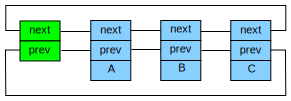
\includegraphics{defer/Linux_list}}
\caption{Linux Circular Linked List (\tco{list})}
\label{fig:defer:Linux Circular Linked List (list)}
\end{figure}

\begin{figure}[tb]
\centering
\resizebox{3in}{!}{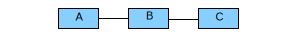
\includegraphics{defer/Linux_list_abbr}}
\caption{Linux Linked List Abbreviated}
\label{fig:defer:Linux Linked List Abbreviated}
\end{figure}

\co{rcu_assign_pointer()} 와 \co{rcu_dereference()} 는 이론적으로 모든 있음직한
RCU 로 보호되는 데이터 구조체를 만들 수 있지만, 실용적으로는 더 높은 수준의
구조물을 사용하는게 나은 경우가 많습니다.
그런 이유로, \co{rcu_assign_pointer()} 와 \co{rcu_dereference()} 기능은
리눅스의 리스트 조정 API 의 특수한 RCU 변종에 내재되었습니다.
리눅스는 두 종류의 양방향 링크드 리스트를 갖는데, 서큘러 \co{struct list_head}
와 리니어 \co{struct hlist_head}/\co{struct hlist_node} 쌍입니다.
전자는
Figure~\ref{fig:defer:Linux Circular Linked List (list)} 에 보인 것과 같이
있는데, (왼쪽의) 초록색 상자는 리스트 헤더를 의미하고 (오른쪽의 세개의) 상자는
이 리스트의 원소들을 의미합니다.
이 표기법은 어색하고, 따라서
Figure~\ref{fig:defer:Linux Linked List Abbreviated} 에 보인 것처럼 헤더가 아닌
(파란색) 원소들만을 보이도록 축약될 겁니다.
\iffalse

Although \co{rcu_assign_pointer()} and
\co{rcu_dereference()} can in theory be used to construct any
conceivable RCU-protected data structure, in practice it is often better
to use higher-level constructs.
Therefore, the \co{rcu_assign_pointer()} and
\co{rcu_dereference()}
primitives have been embedded in special RCU variants of Linux's
list-manipulation API.
Linux has two variants of doubly linked list, the circular
\co{struct list_head} and the linear
\co{struct hlist_head}/\co{struct hlist_node} pair.
The former is laid out as shown in
Figure~\ref{fig:defer:Linux Circular Linked List (list)},
where the green (leftmost) box represent the list header and the blue
(rightmost three) boxes represent the elements in the list.
This notation is cumbersome, and will therefore be abbreviated as shown in
Figure~\ref{fig:defer:Linux Linked List Abbreviated},
which shows only the non-header (blue) elements.
\fi

\begin{figure}[tb]
\centering
\resizebox{3in}{!}{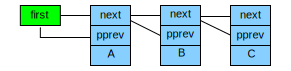
\includegraphics{defer/Linux_hlist}}
\caption{Linux Linear Linked List (\tco{hlist})}
\label{fig:defer:Linux Linear Linked List (hlist)}
\end{figure}

리눅스의 다른 양방향 링크드 리스트, hlist 는 선형 리스트로, 헤더에 순환형
리스트를 위한 두개의 포인터가 아닌 하나의 리스트만 있어도 되는데,
Figure~\ref{fig:defer:Linux Linear Linked List (hlist)} 가 이를 보입니다.
따라서, hlist 의 사용은 커다란 해시 테이블의 해시 bucket 배열의 메모리 사용량을
절반으로 줄일 수 있습니다.
앞에서와 같이, 이 표기법은 다루기 어려우므로, hlist 는 list 와 같이 축약되어
표시될 텐데,
Figure~\ref{fig:defer:Linux Linked List Abbreviated} 와 같습니다.
\iffalse

Linux's other doubly linked list, the hlist,
is a linear list, which means that
it needs only one pointer for the header rather than the two
required for the circular list, as shown in
Figure~\ref{fig:defer:Linux Linear Linked List (hlist)}.
Thus, use of hlist can halve the memory consumption for the hash-bucket
arrays of large hash tables.
As before, this notation is cumbersome, so hlists will be abbreviated
in the same way lists are, as shown in
Figure~\ref{fig:defer:Linux Linked List Abbreviated}.
\fi

% @@@ Refer to \ref{fig:defer:Insertion With Concurrent Readers} and
%	\ref{fig:defer:Deletion With Concurrent Readers}, mostly the latter.

\begin{linelabel}[ln:defer:Canonical RCU Replacement Example (2nd)]
\begin{VerbatimN}[samepage=true,commandchars=\\\[\],firstnumber=15]
q = kmalloc(sizeof(*p), GFP_KERNEL);	\lnlbl[kmalloc]
*q = *p;				\lnlbl[copy]
q->b = 2;				\lnlbl[update1]
q->c = 3;				\lnlbl[update2]
list_replace_rcu(&p->list, &q->list);	\lnlbl[replace]
synchronize_rcu();			\lnlbl[sync_rcu]
kfree(p);				\lnlbl[kfree]
\end{VerbatimN}
\end{linelabel}

\begin{figure}[tbp]
\centering
\resizebox{2.7in}{!}{\includegraphics{defer/RCUReplacement}}
\caption{RCU Replacement in Linked List}
\label{fig:defer:RCU Replacement in Linked List}
\end{figure}

리스트의 초기 상태는 포인터 \co{p} 를 포함해서, 삭제 예제의 것과 동일한데,
Figure~\ref{fig:defer:RCU Replacement in Linked List} 의 첫번째 줄에 보여져
있습니다.
\iffalse

The initial state of the list, including the pointer \co{p},
is the same as for the deletion example, as shown on the
first row of
Figure~\ref{fig:defer:RCU Replacement in Linked List}.
\fi

앞에서와 같이, 각 원소의 세개의 숫자는 필드 \co{a}, \co{b}, 그리고 \co{c} 의
값을 각각 나타내고 있습니다.
빨간색으로 칠해진 원소는 읽기 쓰레드에 의해 레퍼런스 될수도 있고, 읽기 쓰레드는
업데이트 쓰레드와 직접적으로 동기화 하지 않으므로, 읽기 쓰레드는 이 전체 교체
프로세스와 동시에 수행될 수도 있습니다.
여기서도 역방향 포인터와 리스트의 tail 에서 head 로의 링크를 명료성을 위해
생략합니다.

뒤따르는 글은 어떻게 \co{5,6,7} 원소를 \co{5,2,3} 으로 모든 읽기 쓰레드가 이
두개의 값 중 하나만을 보게 하면서 교체하는지 설명합니다.
\iffalse

@@@ As before,
the triples in each element represent the values of fields \co{a},
\co{b}, and \co{c}, respectively.
The red-shaded elements might be referenced by readers,
and because readers do not synchronize directly with updaters,
readers might run concurrently with this entire replacement process.
Please note that
we again omit the backwards pointers and the link from the tail
of the list to the head for clarity.

The following text describes how to replace the \co{5,6,7} element
with \co{5,2,3} in such a way that any given reader sees one of these
two values.
\fi

\begin{lineref}[ln:defer:Canonical RCU Replacement Example (2nd)]
Line~\lnref{kamlloc} 은 교체할 원소를 \co{kmalloc()} 하는데, 이에 따라
Figure~\ref{fig:defer:RCU Replacement in Linked List} 의 두번째 줄의 상태를
초래합니다.
이 시점에서는 어떤 읽기 쓰레드도 이 새로 할당된 원소를 레퍼런스 할 수 없고 (이
사실이 초록색으로 보여져 있습니다), 이 새로 할당된 원소는 초기화 되어있지
않습니다 (물음표로 보여져 있습니다).
\iffalse

Line~\lnref{kmalloc} \co{kmalloc()}s a replacement element, as follows,
resulting in the state as shown in the second row of
Figure~\ref{fig:defer:RCU Replacement in Linked List}.
At this point, no reader can hold a reference to the newly allocated
element (as indicated by its green shading), and it is uninitialized
(as indicated by the question marks).
\fi

Line~\lnref{copy} 는 과거의 원소를 새로운 원소로 복사해서,
Figure~\ref{fig:defer:RCU Replacement in Linked List} 세번째 줄의 상태를
초래합니다.
새로 할당된 원소는 여전히 읽기 쓰레드에 의해 레퍼런스 될 수 없지만, 이제 초기화
되어 있습니다.
\iffalse

Line~\lnref{copy} copies the old element to the new one, resulting in the
state as shown in the third row of
Figure~\ref{fig:defer:RCU Replacement in Linked List}.
The newly allocated element still cannot be referenced by readers, but
it is now initialized.
\fi

Line~\lnref{update1} 은 \co{q->b} 를 값 ``2'' 로 업데이트 하고,
line~\lnref{update2} 는 \co{q->c} 를 값 ``3'' 으로 업데이트 해서,
Figure~\ref{fig:defer:RCU Replacement in Linked List} 의 네번째 줄의 상태를
만듭니다.
\iffalse

Line~\lnref{update1} updates \co{q->b} to the value ``2'', and
line~\lnref{update2} updates \co{q->c} to the value ``3'',
as shown on the fourth row of
Figure~\ref{fig:defer:RCU Replacement in Linked List}.
\fi

이제, line~\lnref{replace} 가 이 교체를 수행해서, 새 원소가 마침내 읽기
쓰레드에게 보여지게 되며, 따라서
Figure~\ref{fig:defer:RCU Replacement in Linked List} 의 다섯째 줄에 보인
것처럼 빨간색으로 칠해집니다.
이 시점에서, 앞에서 본 것처럼, 우린 리스트의 두 버전을 갖습니다.
기존부터 존재한 읽기 쓰레드는 \co{5,6,7} 원소를 볼 수도 있지만 (따라서
노란색으로 칠해져 있습니다), 새로운 읽기 쓰레드는 그대신 \co{5,2,3} 원소를 볼
겁니다.
하지만 어떤 읽기 쓰레드이든 제대로 정의된 리스트를 볼 수 있습니다.
\iffalse

Now, line~\lnref{replace} does the replacement, so that the new element is
finally visible to readers, and hence is shaded red, as shown on
the fifth row of
Figure~\ref{fig:defer:RCU Replacement in Linked List}.
At this point, as shown below, we have two versions of the list.
Pre-existing readers might see the \co{5,6,7} element (which is
therefore now shaded yellow), but
new readers will instead see the \co{5,2,3} element.
But any given reader is guaranteed to see some well-defined list.
\fi

Line~\lnref{sync_rcu} 에서의 \co{synchronize_rcu()} 가 리턴한 후에는, 하나의
grace period 가 지났고, 따라서 \co{list_replace_rcu()} 전에 시작된 모든 읽기
쓰레드는 완료되었습니다.
특히, \co{5,6,7} 원소로의 레퍼런스를 쥐고 있었을 수 있는 모든 읽기 쓰레드는
그것들의 RCU read-side 크리티컬 섹션을 빠져나왔을 것이 보장되며, 따라서
레퍼런스를 계속 가지고 있는게 금지되었습니다.
따라서, 과거의 원소로의 레퍼런스를 가지고 있는 읽기 쓰레드는 더이상 존재하지
않는데,
Figure~\ref{fig:defer:RCU Replacement in Linked List} 의 여섯번째 줄에
초록색으로 표시되었습니다.
읽기 쓰레드들이 생각하기로, 우리는 리스트의 하나의 버전으로 돌아왔습니다만,
새로운 원소가 기존 것의 위치에 있게 되었습니다.
\iffalse

After the \co{synchronize_rcu()} on line~\lnref{sync_rcu} returns,
a grace period will have elapsed, and so all readers that started before the
\co{list_replace_rcu()} will have completed.
In particular, any readers that might have been holding references
to the \co{5,6,7} element are guaranteed to have exited
their RCU read-side critical sections, and are thus prohibited from
continuing to hold a reference.
Therefore, there can no longer be any readers holding references
to the old element, as indicated its green shading in the sixth row of
Figure~\ref{fig:defer:RCU Replacement in Linked List}.
As far as the readers are concerned, we are back to having a single version
of the list, but with the new element in place of the old.
\fi

Line~\lnref{kfree} 에서의 \co{kfree()} 가 완료되면, 이 리스트는
Figure~\ref{fig:defer:RCU Replacement in Linked List}
의 마지막 줄에 보인 것처럼 됩니다.
\iffalse

After the \co{kfree()} on line~\lnref{kfree} completes, the list will
appear as shown on the final row of
Figure~\ref{fig:defer:RCU Replacement in Linked List}.
\fi
\end{lineref}

RCU 가 이 교체 경우에 의해 이름지어졌긴 하지만, 리눅스 커널 내에서의 많은 RCU
사용 경우는
Section~\ref{sec:defer:Maintain Multiple Versions of Recently Updated Objects}
에 보인 간단한 삭제의 경우에 의존합니다.
\iffalse

Despite the fact that RCU was named after the replacement case,
the vast majority of RCU usage within the Linux kernel relies on
the simple deletion case shown in
Section~\ref{sec:defer:Maintain Multiple Versions of Recently Updated Objects}.
\fi

\begin{sidewaystable*}[htbp]
\rowcolors{1}{}{lightgray}
\renewcommand*{\arraystretch}{1.3}
\centering
\caption{RCU-Protected List APIs}
\label{tab:defer:RCU-Protected List APIs}
\footnotesize
\newlength{\cwa}\newlength{\cwb}\newlength{\cwc}\newlength{\cwd}
\IfNimbusAvail{
  \renewcommand{\ttdefault}{NimbusMonoN}
  \setlength{\cwa}{1.9in}\setlength{\cwb}{2.1in}
  \setlength{\cwc}{1.8in}\setlength{\cwd}{1.6in}
}{
  \setlength{\cwa}{1.95in}\setlength{\cwb}{2.15in}
  \setlength{\cwc}{1.9in}\setlength{\cwd}{1.7in}
}
\begin{tabular}{>{\raggedright\arraybackslash}p{\cwa}
    >{\raggedright\arraybackslash}p{\cwb}
    >{\raggedright\arraybackslash}p{\cwc}
    >{\raggedright\arraybackslash}p{\cwd}}
\toprule
\pmb{\tco{list}}: Circular doubly linked list &
    \pmb{\tco{hlist}}: Linear doubly linked list &
	\pmb{\tco{hlist_nulls}}: Linear doubly linked list with marked
	NULL pointer, with up to 31~bits of marking &
	    \pmb{\tco{hlist_bl}}: Linear doubly linked list with bit locking \\
\midrule
\multicolumn{4}{l}{{\bf Initialization}} \\
&
    \tco{INIT_LIST_HEAD_RCU()} &
	&
	    \\
\multicolumn{4}{l}{{\bf Full traversal}} \\
\tco{list_for_each_entry_rcu()}
\tco{list_for_each_entry_lockless()} &
    \tco{hlist_for_each_entry_rcu()}
    \tco{hlist_for_each_entry_rcu_bh()}
    \tco{hlist_for_each_entry_rcu_notrace()} &
	\tco{hlist_nulls_for_each_entry_rcu()}
	\tco{hlist_nulls_for_each_entry_safe()} &
	    \tco{hlist_bl_for_each_entry_rcu()} \\
\multicolumn{4}{l}{{\bf Resume traversal}} \\
\tco{list_for_each_entry_continue_rcu()}
\tco{list_for_each_entry_from_rcu()} &
    \tco{hlist_for_each_entry_continue_rcu()}
    \tco{hlist_for_each_entry_continue_rcu_bh()}
    \tco{hlist_for_each_entry_from_rcu()} &
	&
	    \\
\multicolumn{4}{l}{{\bf Stepwise traversal}} \\
\tco{list_entry_rcu()}
\tco{list_entry_lockless()}
\tco{list_first_or_null_rcu()}
\tco{list_next_rcu()}
\tco{list_next_or_null_rcu()} &
    \multicolumn{1}{p{1.2in}}{\tco{hlist_first_rcu()}
			      \tco{hlist_next_rcu()}
			      \tco{hlist_pprev_rcu()}} &
	\tco{hlist_nulls_first_rcu()}
	\tco{hlist_nulls_next_rcu()} &
	    \tco{hlist_bl_first_rcu()} \\
\multicolumn{4}{l}{{\bf Add}} \\
\multicolumn{1}{p{1.2in}}{\tco{list_add_rcu()}
			  \tco{list_add_tail_rcu()}} &
    \tco{hlist_add_before_rcu()}
    \tco{hlist_add_behind_rcu()}
    \tco{hlist_add_head_rcu()}
    \tco{hlist_add_tail_rcu()} &
	\tco{hlist_nulls_add_head_rcu()} &
	    \tco{hlist_bl_add_head_rcu()}
	    \tco{hlist_bl_set_first_rcu()} \\
\multicolumn{4}{l}{{\bf Delete}} \\
\tco{list_del_rcu()} &
    \multicolumn{1}{p{1.2in}}{\tco{hlist_del_rcu()}
			      \tco{hlist_del_init_rcu()}} &
	\tco{hlist_nulls_del_rcu()}
	\tco{hlist_nulls_del_init_rcu()} &
	    \tco{hlist_bl_del_rcu()}
	    \tco{hlist_bl_del_init_rcu()} \\
\multicolumn{4}{l}{{\bf Replace}} \\
\tco{list_replace_rcu()} &
    \tco{hlist_replace_rcu()} &
	&
	    \\
\multicolumn{4}{l}{{\bf Splice}} \\
\tco{list_splice_init_rcu()} &
    \tco{list_splice_tail_init_rcu()} &
	&
	    \\
\bottomrule
\end{tabular}
\end{sidewaystable*}

The first pair of categories operate on Linux
\co{struct list_head} lists, which are circular, doubly-linked
lists.
The \co{list_for_each_entry_rcu()} primitive traverses an
RCU-protected list in a type-safe manner, while also enforcing
memory ordering for situations where a new list element is inserted
into the list concurrently with traversal.
On non-Alpha platforms, this primitive incurs little or no performance
penalty compared to \co{list_for_each_entry()}.
The \co{list_add_rcu()}, \co{list_add_tail_rcu()},
and \co{list_replace_rcu()} primitives are analogous to
their non-RCU counterparts, but incur the overhead of an additional
memory barrier on weakly-ordered machines.
The \co{list_del_rcu()} primitive is also analogous to its
non-RCU counterpart, but oddly enough is very slightly faster due to the
fact that it poisons only the \co{prev} pointer rather than
both the \co{prev} and \co{next} pointers as
\co{list_del()} must do.
Finally, the \co{list_splice_init_rcu()} primitive is similar
to its non-RCU counterpart, but incurs a full grace-period latency.
The purpose of this grace period is to allow RCU readers to finish
their traversal of the source list before completely disconnecting
it from the list header---failure to do this could prevent such
readers from ever terminating their traversal.

\QuickQuiz{}
	\co{list_del_rcu()} 는 왜 \co{next} 와 \co{prev} 두 포인터를 모두
	파괴하지 않는거죠?
	\iffalse

	Why doesn't \co{list_del_rcu()} poison both the \co{next}
	and \co{prev} pointers?
	\fi
\QuickQuizAnswer{
	\co{next} 포인터를 파괴하는 행위는 이 포인터를 사용해야 하는 동시의 RCU
	읽기 쓰레드들과 간섭될 수 있습니다.
	하지만, RCU 읽기 쓰레드들은 \co{prev} 포인터의 사용으로부터 숨겨져
	있으므로 이건 안전하게 파괴될 수 있습니다.
	\iffalse

	Poisoning the \co{next} pointer would interfere
	with concurrent RCU readers, who must use this pointer.
	However, RCU readers are forbidden from using the \co{prev}
	pointer, so it may safely be poisoned.
	\fi
} \QuickQuizEnd

다음의 두 카테고리는 리눅스의 선형 링크드 리스트인 \co{struct hlist_head} 에
대해 동작합니다.
\co{struct list_head} 에 비해 \co{struct hlist_head} 의 장점은 하나의 포인터를
갖는 리스트 헤더만이 필요해서 커다란 해시 테이블에서는 상당한 양의 메모리를
아낄 수 있다는 점입니다.
이 표에서의 \co{struct hlist_head} 의 기능들과 RCU 를 사용하지 않는 비슷한
것들과의 관계는 \co{struct list_head} 기능들이 그러한 것과 거의 같습니다.
\iffalse

The second pair of categories operate on Linux's
\co{struct hlist_head}, which is a linear linked list.
One advantage of \co{struct hlist_head} over
\co{struct list_head} is that the former requires only
a single-pointer list header, which can save significant memory in
large hash tables.
The \co{struct hlist_head} primitives in the table
relate to their non-RCU counterparts in much the same way as do the
\co{struct list_head} primitives.
\fi

The next section looks at APIs that assist developers in debugging
their code that makes use of RCU.

\subsubsection{RCU Has Diagnostic APIs}
\label{sec:defer:RCU Has Diagnostic APIs}

\begin{table}[tb]
\renewcommand*{\arraystretch}{1.15}
\footnotesize
\centering
\begin{tabular}{ll}
\toprule
Category &
	Primitives \\
\midrule
Mark RCU pointer &
	\tco{__rcu} \\
\midrule
Debug-object support &
	\tco{init_rcu_head()} \\
&	\tco{destroy_rcu_head()} \\
&	\tco{init_rcu_head_on_stack()} \\
&	\tco{destroy_rcu_head_on_stack()} \\
\midrule
Stall-warning control &
	\tco{rcu_cpu_stall_reset()} \\
\midrule
Callback checking &
	\tco{rcu_head_init()} \\
&	\tco{rcu_head_after_call_rcu()} \\
\midrule
lockdep support &
	\tco{rcu_read_lock_held()} \\
&	\tco{rcu_read_lock_bh_held()} \\
&	\tco{rcu_read_lock_sched_held()} \\
&	\tco{srcu_read_lock_held()} \\
&	\tco{rcu_is_watching()} \\
&	\tco{RCU_LOCKDEP_WARN()} \\
&	\tco{RCU_NONIDLE()} \\
&	\tco{rcu_sleep_check()} \\
\bottomrule
\end{tabular}
\caption{RCU Diagnostic APIs}
\label{tab:defer:RCU Diagnostic APIs}
\end{table}

Table~\ref{tab:defer:RCU Diagnostic APIs}
은 RCU 의 검사 API 들을 보입니다.
\iffalse

Table~\ref{tab:defer:RCU Diagnostic APIs}
shows RCU's diagnostic APIs.
\fi

\co{__rcu} 는 RCU 로 보호되는 포인터를 마킹하는데, 예를 들어, \qco{strcut foo
__rcu *p;} 같은 식입니다.
\co{rcu_dereference()} 로 전달될 수도 있는 포인터들이 마킹될 수 있습니다만,
\co{rcu_dereference()} 로부터 리턴되는 값을 잡고 있는 포인터는 그러지 않아도
됩니다.
이 마킹을 변수, 구조체 필드, 함수 패러미터, 그리고 리턴 값에 가하는 것은 리눅스
커널의 \co{sparse} 도구가 RCU 로 보호되는 포인터가 올바르지 않게도 평범한
C-언어 로드와 스토어로 접근되는 것을 알 수 있게 해줍니다.
\iffalse

The \co{__rcu} marks an RCU-protected pointer, for example,
\qco{struct foo __rcu *p;}.
Pointers that might be passed to \co{rcu_dereference()} can be marked,
but pointers holding values returned from \co{rcu_dereference()}
should not be.
Providing these markings on variables, structure fields, function
parameters, and return values allows the Linux kernel's \co{sparse}
tool to detect situtations where RCU-protected pointers are
incorrectly accessed using plain C-language loads and stores.
\fi

리눅스 커널의 메모리 할당자로부터 얻어지는 구조체의 \co{rcu_head} 구조체 부분은
자동으로 디버그 오브젝트 지원을 받습니다만, 스스로의 특수 목적 메모리 할당자를
만든 것들은 할당과 해제 시에 각각 \co{init_rcu_head()} 와
\co{destroy_rcu_head()} 를 사용할 수 있습니다.
함수 호출 스택에서 할당된 \co{rcu_head} 를 사용하는 경우 (진짜 이런 경우가
있습니다!) 에는 첫 접근 전에 \co{init_rcu_head_on_stack()} 을, 마지막 접근
후에, 그러나 그 함수에서 리턴하기 전에 \co{destroy_rcu_head_on_stack()} 을
사용할 수 있습니다.
디버그 오브젝트 지원은 같은 \co{rcu_head} 구조체를 \co{call_rcu()} 와 그 유사한
것들에 보내는 경우를 파악할 수 있게 합니다, 이것은 유명한 double-free 클래스
버그의 \co{call_rcu()} 버전이죠.
\iffalse

Debug-object support is automatic for any \co{rcu_head} structures
that are part of a structure obtained from the Linux kernel's
memory allocators, but those building their own special-purpose
memory allocators can use \co{init_rcu_head()} and \co{destroy_rcu_head()}
at allocation and free time, respectively.
Those using \co{rcu_head} structures allocated on the function-call
stack (it happens!) may use \co{init_rcu_head_on_stack()}
before first use and \co{destroy_rcu_head_on_stack()} after last use,
but before returning from the function.
Debug-object support allows detection of bugs involving passing the
same \co{rcu_head} structure to \co{call_rcu()} and friends in
quick succession, which is the \co{call_rcu()} counterpart to the
infamous double-free class of bugs.
\fi

스톨 경고 제어는 \co{rcu_cpu_stall_reset()} 으로 제공되는데, 이는 호출자가 현재
grace period 의 남은 기간 동안 RCU CPU 스톨 경고를 내지 않게끔 합니다.
RCU CPU 스톨 경고는 RCU read-side 크리티컬 섹션이 지나치게 긴 시간 동안
수행되는 상황을 집어낼 수 있게 도와주며, 커널 디버거와 같은 것들이
브레이크포인트를 마주치거나 하는 경우에 이 경고를 막을 수 있게 하는게
유용합니다.
\iffalse

Stall-warning control is provided by \co{rcu_cpu_stall_reset()}, which
allows the caller to suppress RCU CPU stall warnings for the remainder
of the current grace period.
RCU CPU stall warnings help pinpoint situations where an RCU read-side
critical section runs for an excessive length of time, and it is useful
for things like kernel debuggers to be able to suppress them, for example,
when encountering a breakpoint.
\fi

콜백 체크는 \co{rcu_head_init()} 와 \co{rcu_head_after_call_rcu()} 를 통해
제공됩니다.
앞의 것은 \co{rcu_head} 구조체에 의해, \co{call_rcu()} 에 이 구조체가 넘겨지기
전에 수행되고, \co{rcu_head_after_call_rcu()} 는 이 콜백이 명시된 함수와 함께
수행되었는지 체크합니다.
\iffalse

Callback checking is provided by \co{rcu_head_init()} and
\co{rcu_head_after_call_rcu()}.
The former is invoked on an \co{rcu_head} structure before it is passed
to \co{call_rcu()}, and then \co{rcu_head_after_call_rcu()} will
check to see if the callback is has been invoked with the specified
function.
\fi

Lockdep~\cite{JonathanCorbet2006lockdep} 을 위한 지원이
\co{rcu_read_lock_held()},
\co{rcu_read_lock_bh_held()},
\co{rcu_read_lock_sched_held()}, 그리고
\co{srcu_read_lock_held()} 에 포함되어 있는데, 이것들 각각은 연관된 RCU
read-side 크리티컬 섹션 타입 내에서 실행된 경우 \co{true} 를 리턴합니다.
\iffalse

Support for lockdep~\cite{JonathanCorbet2006lockdep} includes
\co{rcu_read_lock_held()},
\co{rcu_read_lock_bh_held()},
\co{rcu_read_lock_sched_held()}, and
\co{srcu_read_lock_held()},
each of which returns \co{true} if invoked within the corresponding
type of RCU read-side critical section.
\fi

\QuickQuiz{}
	Tasks RCU 를 위한 \co{rcu_read_lock_tasks()} 는 왜 없나요?
	\iffalse

	Why isn't there a \co{rcu_read_lock_tasks()} for Tasks RCU?
	\fi
\QuickQuizAnswer{
	Tasks RCU 는 read-side 마커가 없기 때문입니다.
	그대신, Tasks RCU read-side 크리티컬 섹션은 자발적인 컨텍스트 스위치로
	제한됩니다.
	\iffalse

	Because Tasks RCU does not have read-side markers.
	Instead, Tasks RCU read-side critical sections are
	bounded by voluntary context switches.
	\fi
} \QuickQuizEnd

\co{rcu_read_lock()} 은 idle 루프 내에서 사용될 수 없기 때문에, 그리고 에너지
효율성에 대한 고려가 이 idle 루프가 지나치게 장식되게 했기 때문에,
\co{rcu_is_watching()} 은 \co{rcu_read_lock()} 의 사용이 합법적인 컨텍스트에서
호출된 경우 true 를 리턴합니다.
\co{srcu_read_lock()} 은 idle 에서, 그리고 심지어 오프라인 CPU 에서도 호출될 수
있음을 다시 말씀드리는데, 이는 \co{rcu_is_watching()} 은 SRCU 에 적용되지
않음을 의미합니다.
\iffalse

Because \co{rcu_read_lock()} cannot be used from the idle loop,
and because energy-efficiency concerns have caused the idle loop
to become quite ornate, \co{rcu_is_watching()} returns true if
invoked in a context where use of \co{rcu_read_lock()} is legal.
Note again that \co{srcu_read_lock()} may be used from idle and
even offline CPUs, which means that \co{rcu_is_watching()} does not
apply to SRCU.
\fi

\co{RCU_LOCKDEP_WARN()} 은 lockdep 이 활성화 되어 있고 그 인자가 \co{true} 로
평가되면 경고를 냅니다.
예를 들어, \co{RCU_LOCKDEP_WARN(!rcu_read_lock_held())} 는 RCU read-side
크리티컬 섹션 외에서 호출되었다면 경고를 내놓을 겁니다.
\iffalse

\co{RCU_LOCKDEP_WARN()} emits a warning if lockdep is enabled and if
its argument evaluated to \co{true}.
For example, \co{RCU_LOCKDEP_WARN(!rcu_read_lock_held())} would emit a
warning if invoked outside of an RCU read-side critical section.
\fi

\co{RCU_NONIDLE()} 은 RCU 가 전체 인자로 넘어온 문장을 수행하는 시점을 보게
강제하는데 사용될 수 있을 겁니다.
예를 들어, \co{RCU_NONIDLE(WARN_ON(!rcu_is_watching()))} 은 결코 경고를 내지
않을 겁니다.

마지막으로, \co{rcu_sleep_check()} 는 RCU, RCU-bh, 또는 RCU-sched read-side
크리티컬 섹션 내에서 호출되었을 때 경고를 내놓습니다.
\iffalse

\co{RCU_NONIDLE()} may be used to force RCU to watch when executing
the statement that is passed in as the sole argument.
For example, \co{RCU_NONIDLE(WARN_ON(!rcu_is_watching()))}
would never emit a warning.

Finally,  \co{rcu_sleep_check()} emits a warning if invoked within
an RCU, RCU-bh, or RCU-sched read-side critical section.
\fi

\subsubsection{Where Can RCU's APIs Be Used?}
\label{sec:defer:Where Can RCU's APIs Be Used?}

\begin{figure}[tb]
\begin{center}
\resizebox{3in}{!}{\includegraphics{defer/RCUenvAPI}}
\end{center}
\caption{RCU API Usage Constraints}
\label{fig:defer:RCU API Usage Constraints}
\end{figure}

Figure~\ref{fig:defer:RCU API Usage Constraints}
는 커널 내의 어떤 환경에서 어떤 API 들이 사용될 수 있는지 보입니다.
RCU read-side 기능은 NMI를 포함해 어떤 환경에서도 사용될 수 있고, RCU 의 변경
기능과 비동기적인 grace-period 기능은 NMI 를 제외한 모든 환경에서 사용될 수
있으며, RCU 의 동기적인 grace-period 기능은 프로세스 컨텍스트에서만 사용될 수
있습니다.
RCU 리스트 횡단 기능은 \co{list_for_each_entry_rcu()},
\co{hlist_for_each_entry_rcu()} 등을 포함합니다.
비슷하게, RCU list 변경 기능은 \co{list_add_rcu()}, \co{hlist_del_rcu()} 등을
포함합니다.

다른 종류의 RCU 로부터의 기능은 대체될 수도 있는데, 예를 들어
\co{srcu_read_lock()} 은 \co{rcu_read_lock()} 이 사용될 수 있는 모든
컨텍스트에서 사용될 수 있습니다.
\iffalse

Figure~\ref{fig:defer:RCU API Usage Constraints}
shows which APIs may be used in which in-kernel environments.
The RCU read-side primitives may be used in any environment, including NMI,
the RCU mutation and asynchronous grace-period primitives may be used in any
environment other than NMI, and, finally, the RCU synchronous grace-period
primitives may be used only in process context.
The RCU list-traversal primitives include \co{list_for_each_entry_rcu()},
\co{hlist_for_each_entry_rcu()}, etc.
Similarly, the RCU list-mutation primitives include
\co{list_add_rcu()}, \co{hlist_del_rcu()}, etc.

Note that primitives from other families of RCU may be substituted,
for example, \co{srcu_read_lock()} may be used in any context
in which \co{rcu_read_lock()} may be used.
\fi

\subsubsection{So, What \emph{is} RCU Really?}
\label{sec:defer:So, What is RCU Really?}

그 핵심에 있어서, RCU 는 더도 덜도 아니고 데이터 삽입의 공개와 구독을 지원하고
모든 RCU 읽기 쓰레드들이 완료되길 기다리며, 여러 버전들을 관리하는 API 입니다.
그렇다곤 하나, RCU 위에 reader-writer 락킹, 레퍼런스 카운팅, 그리고
Section~\ref{sec:defer:RCU Usage} 에서 열거한 존재 보장과 같은 고차원의 것들을
만드는 것이 가능합니다.
더 나아가서, 리눅스 커뮤니티가 RCU 의 흥미롭고 새로운 사용처를 찾을 것이라 믿어
의심치 않습니다, 커널의 여러 동기화 기능들에 대해서 그랬듯이요.

물론, 더 완벽한 RCU 에 대한 이해는 이 API 들을 가지고 할 수 있는 일에 대한
것들도 포함할 것입니다.

하지만, 많은 사람들의 경우 RCU 에 대한 완벽한 이해에는 RCU 구현의 예가 포함될
겁니다.
따라서 Appendix~\ref{chp:app:``Toy'' RCU Implementations} 는 복잡도와 기능성을
늘려가는 일련의 ``장난감'' RCU 구현들을 소개합니다, 다른 사람들은 고전적인
``User-Level Read-Copy Update 구현''~\cite{MathieuDesnoyers2012URCU} 을 더
선호할 수도 있겠지만요.
그렇지 않은 모두를 위해, 다음 섹션은 학계와 산업계에서의 RCU 사용에 대한 개괄을
제공합니다.
\iffalse

At its core, RCU is nothing more nor less than an API that supports
publication and subscription for insertions, waiting for all RCU readers
to complete, and maintenance of multiple versions.
That said, it is possible to build higher-level constructs
on top of RCU, including the reader-writer-locking, reference-counting,
and existence-guarantee constructs listed in
Section~\ref{sec:defer:RCU Usage}.
Furthermore, I have no doubt that the Linux community will continue to
find interesting new uses for RCU,
just as they do for any of a number of synchronization
primitives throughout the kernel.

Of course, a more-complete view of RCU would also include
all of the things you can do with these APIs.

However, for many people, a complete view of RCU must include sample
RCU implementations.
Appendix~\ref{chp:app:``Toy'' RCU Implementations} therefore presents a series
of ``toy'' RCU implementations of increasing complexity and capability,
though others might prefer the classic
``User-Level Implementations of Read-Copy
Update''~\cite{MathieuDesnoyers2012URCU}.
For everyone else, the next section gives an overview of some RCU use cases.
\fi
